\documentclass{article}
\usepackage[utf8]{inputenc}
\newcommand{\ii}{{\bf i}}
\newcommand{\jj}{{\bf j}}
\newcommand{\kk}{{\bf k}}
\newcommand{\id}{{\bf 1}}
\newcommand{\hur}{\frac{\id+\ii+\jj+\kk}{2}}%The "Hurwitz point"
\newcommand{\hurwitz}{\Z\left[\hur,\ii,\jj,\kk\right]}%The set of Hurwitz integers
\usepackage{wrapfig}
\usepackage{calligra}
\usepackage[utf8]{inputenc}
\usepackage[dvips]{graphicx}
\usepackage{a4wide}
\usepackage{amsmath}
\usepackage{euscript}
\usepackage{amssymb}
\usepackage{amsthm}
\usepackage{amsopn}
\usepackage[colorinlistoftodos]{todonotes}
\usepackage{graphicx}
\usepackage[T1]{fontenc}
\newcommand\mybar{\kern1pt\rule[-\dp\strutbox]{.8pt}{\baselineskip}\kern1pt}

\usepackage{ulem}
\usepackage{xcolor}
\newcommand{\cs}[1]{\color{blue}{#1}\normalcolor}

%Matrix commands
\newcommand{\ba}{\begin{array}}
\newcommand{\ea}{\end{array}}
\newcommand{\bmat}{\left[\begin{array}}
\newcommand{\emat}{\end{array}\right]}
\newcommand{\bdet}{\left|\begin{array}}
\newcommand{\edet}{\end{array}\right|}
\newcommand{\inv}[1]{#1^{-1}}

%Environment commands
\newcommand{\be}{\begin{enumerate}}
\newcommand{\ee}{\end{enumerate}}
\newcommand{\bi}{\begin{itemize}}
\newcommand{\ei}{\end{itemize}}
\newcommand{\bt}{\begin{thm}}
\newcommand{\et}{\end{thm}}
\newcommand{\bp}{\begin{proof}}
\newcommand{\ep}{\end{proof}}
\newcommand{\bprop}{\begin{prop}}
\newcommand{\eprop}{\end{prop}}
\newcommand{\bl}{\begin{lemma}}
\newcommand{\el}{\end{lemma}}
\newcommand{\bc}{\begin{cor}}
\newcommand{\ec}{\end{cor}}
\newcommand{\lcm}{\mbox{lcm}}
\newcommand{\defn}{\fbox{definition}}
\newcommand{\prop}{\fbox{proposition}}
\newcommand{\stab}{\mbox{stab}}
\newcommand{\Aut}{\mbox{Aut}}
\newcommand{\orb}{\mbox{orb}}

\newcommand{\norm}{\righttriangle}

\newcommand{\and}{\wedge}
\newcommand{\or}{\vee}



%sets of numbers
\newcommand{\N}{\mathbb{N}}
\newcommand{\Z}{\mathbb{Z}}
\newcommand{\Q}{\mathbb{Q}}
\newcommand{\R}{\mathbb{R}}

\newcommand{\topT}{\mathcal{T}}
\newcommand{\standtop}{\mathcal{T}_{STD}}
\newcommand{\cc}{\mathcal{C}}


\documentclass{article}
\usepackage[utf8]{inputenc}
\newcommand{\ii}{{\bf i}}
\newcommand{\jj}{{\bf j}}
\newcommand{\kk}{{\bf k}}
\newcommand{\id}{{\bf 1}}
\newcommand{\hur}{\frac{\id+\ii+\jj+\kk}{2}}%The "Hurwitz point"
\newcommand{\hurwitz}{\Z\left[\hur,\ii,\jj,\kk\right]}%The set of Hurwitz integers
\usepackage{wrapfig}
\usepackage{calligra}
\usepackage[utf8]{inputenc}
\usepackage[dvips]{graphicx}
\usepackage{a4wide}
\usepackage{amsmath}
\usepackage{euscript}
\usepackage{amssymb}
\usepackage{amsthm}
\usepackage{amsopn}
\usepackage[colorinlistoftodos]{todonotes}
\usepackage{graphicx}
\usepackage[T1]{fontenc}
\newcommand\mybar{\kern1pt\rule[-\dp\strutbox]{.8pt}{\baselineskip}\kern1pt}

\usepackage{ulem}
\usepackage{xcolor}
\newcommand{\cs}[1]{\color{blue}{#1}\normalcolor}

%Matrix commands
\newcommand{\ba}{\begin{array}}
\newcommand{\ea}{\end{array}}
\newcommand{\bmat}{\left[\begin{array}}
\newcommand{\emat}{\end{array}\right]}
\newcommand{\bdet}{\left|\begin{array}}
\newcommand{\edet}{\end{array}\right|}
\newcommand{\inv}[1]{#1^{-1}}

%Environment commands
\newcommand{\be}{\begin{enumerate}}
\newcommand{\ee}{\end{enumerate}}
\newcommand{\bi}{\begin{itemize}}
\newcommand{\ei}{\end{itemize}}
\newcommand{\bt}{\begin{thm}}
\newcommand{\et}{\end{thm}}
\newcommand{\bp}{\begin{proof}}
\newcommand{\ep}{\end{proof}}
\newcommand{\bprop}{\begin{prop}}
\newcommand{\eprop}{\end{prop}}
\newcommand{\bl}{\begin{lemma}}
\newcommand{\el}{\end{lemma}}
\newcommand{\bc}{\begin{cor}}
\newcommand{\ec}{\end{cor}}
\newcommand{\lcm}{\mbox{lcm}}
\newcommand{\defn}{\fbox{definition}}
\newcommand{\prop}{\fbox{proposition}}
\newcommand{\stab}{\mbox{stab}}
\newcommand{\Aut}{\mbox{Aut}}
\newcommand{\orb}{\mbox{orb}}

\newcommand{\norm}{\righttriangle}

\newcommand{\and}{\wedge}
\newcommand{\or}{\vee}



%sets of numbers
\newcommand{\N}{\mathbb{N}}
\newcommand{\Z}{\mathbb{Z}}
\newcommand{\Q}{\mathbb{Q}}
\newcommand{\R}{\mathbb{R}}

\newcommand{\topT}{\mathcal{T}}
\newcommand{\standtop}{\mathcal{T}_{STD}}
\newcommand{\cc}{\mathcal{C}}


\title{Topology}
\author{August bergquist}


\begin{document}

\maketitle
\fbox{Theorem 7.17}\\
 If $X$ is compact and $f:X\rightarrow Y$ is continuous and surjective, then $Y$ is compact.\\

\fbox{proof} Suppose by way of contradiction that $X$ is compact, and $f:X\rightarrow Y$ is continuous and surjective, while $Y$ is not compact. Since $Y$ is not compact, there exists some open cover of $Y$ which does not have an open subcover. Call this $\mathcal{C}_Y$. Let $\mathcal{C}_X$ be the set of all inverse images of elements of $\mathcal{C}_Y$. Notice that this is an open cover of $\mathcal{C}_Y$ (since its members are open by definition of continuity). Suppose that this did have a finite subcover. Then the union of those elements would cover $X$, and since it's surjective, the union of their images should cover $Y$, contradicting the fact that $\mathcal{C}_Y$ has no finite subcover.\\

\fbox{Theorem 7.26} Show that homeomorphism is an equivalence relation.\\

\\

\fbox{proof} To show that homeomorphism is an equivalence relation on the set of all topological spaces, we will need to show (1) that it is reflexive, (2) that it is symmetric, (3) that it is transitive. Let $(X,\topT_X)$, $(Y, \topT_Y)$ and $(Z,\topT_Z)$ be arbitrary topological spaces. For fun, let $\cong$ denote homeomorphicness.
\begin{enumerate}
    \item To show that $(X,\topT_X)\cong (X,\topT_X)$, consider the identity map $1_X:X\rightarrow X$. The identity map is bijective, as we know from foudnations, and its inverse is itself. Furthermore, consider some arbitrary $U$ in $\topT_X$. Then the inverse image of $U$ is just $U$, which is still in $\topT_X$. Hence the identity map is continuous. Since it is its own inverse, its inverse is also continuous. Hence $1_X$ is a homomorphism from $X$ to $X$, and $(X,\topT_X)\cong (X,\topT_X)$.
    \item Suppose now that $(X,\topT_X)\cong (Y,\topT_Y)$. Then by definition of homeomorphicness it follows that there exists some continuous bijection $f:X\rightarrow Y$ whose inverse $\inv{f}:Y\rightarrow X$ is also continuous. Recall from foundations that the inverse of a bijective function is bijective, hence $\inv{f}$ is also a bijection. Furthermore, by construction of $\inv{f}$ is also continuous. It's inverse is $f$, and by construction this is continuous. Hence by definition of a homeomorphism, $\inv{f}:Y\rightarrow X$ is a homeomorphism. Since there exists a homeomorphism from $Y$ to $X$, it follows that $(Y,\topT_Y)\cong(X,\topT_X)$.
    \item Suppose that 
\end{enumerate}


\fbox{Exercise 2.27} Let $a$ and $b$ be points of $\R$ such that $a > b$. Show that $(a,b)$ with the subspace topology from $\R_{std}$ is homeomorphic to $\R_{std}$.\\

\fbox{proof 1} Consider the function $f:(a,b)\rightarrow \R$ defined $f(x) = (a-b)/2(1/(a-x))-1$ for all $x\in (a,b)$ where $x > (a-b)/2$, $f(x) = (a-b)/2(1/(b-x)) - 1$ for all $x\in (a,b)$ where $x < (a-b)/2$, and $f(x) = 0$ when $x = (a-b)/2$. Notice that this function is continuous in the standard topology, as we know from calculus. The function also passes the horizontal line test if we graph it, and has positive and negative asymptotes at $a$ and $b$, so every real number is reached. The inverse of this function is also continuous, we could verify from calculus. We could also verify this more rigorously, but I'll leave that for in-class.\\

\fbox{proof 2} This isn't a proof in the strictest sense, but it is kind of cool. Place a circle on top of the real line, whose center is exactly above the origin. Now cut the interval in half, where the top of the circle represents both $a$ and $b$. Drawing tangents on the circle facing away from the top, where these tangents intersect the real-line is the output of the function $f$. This is a homeomorphism.

\begin{figure}[htbp]
\centerline{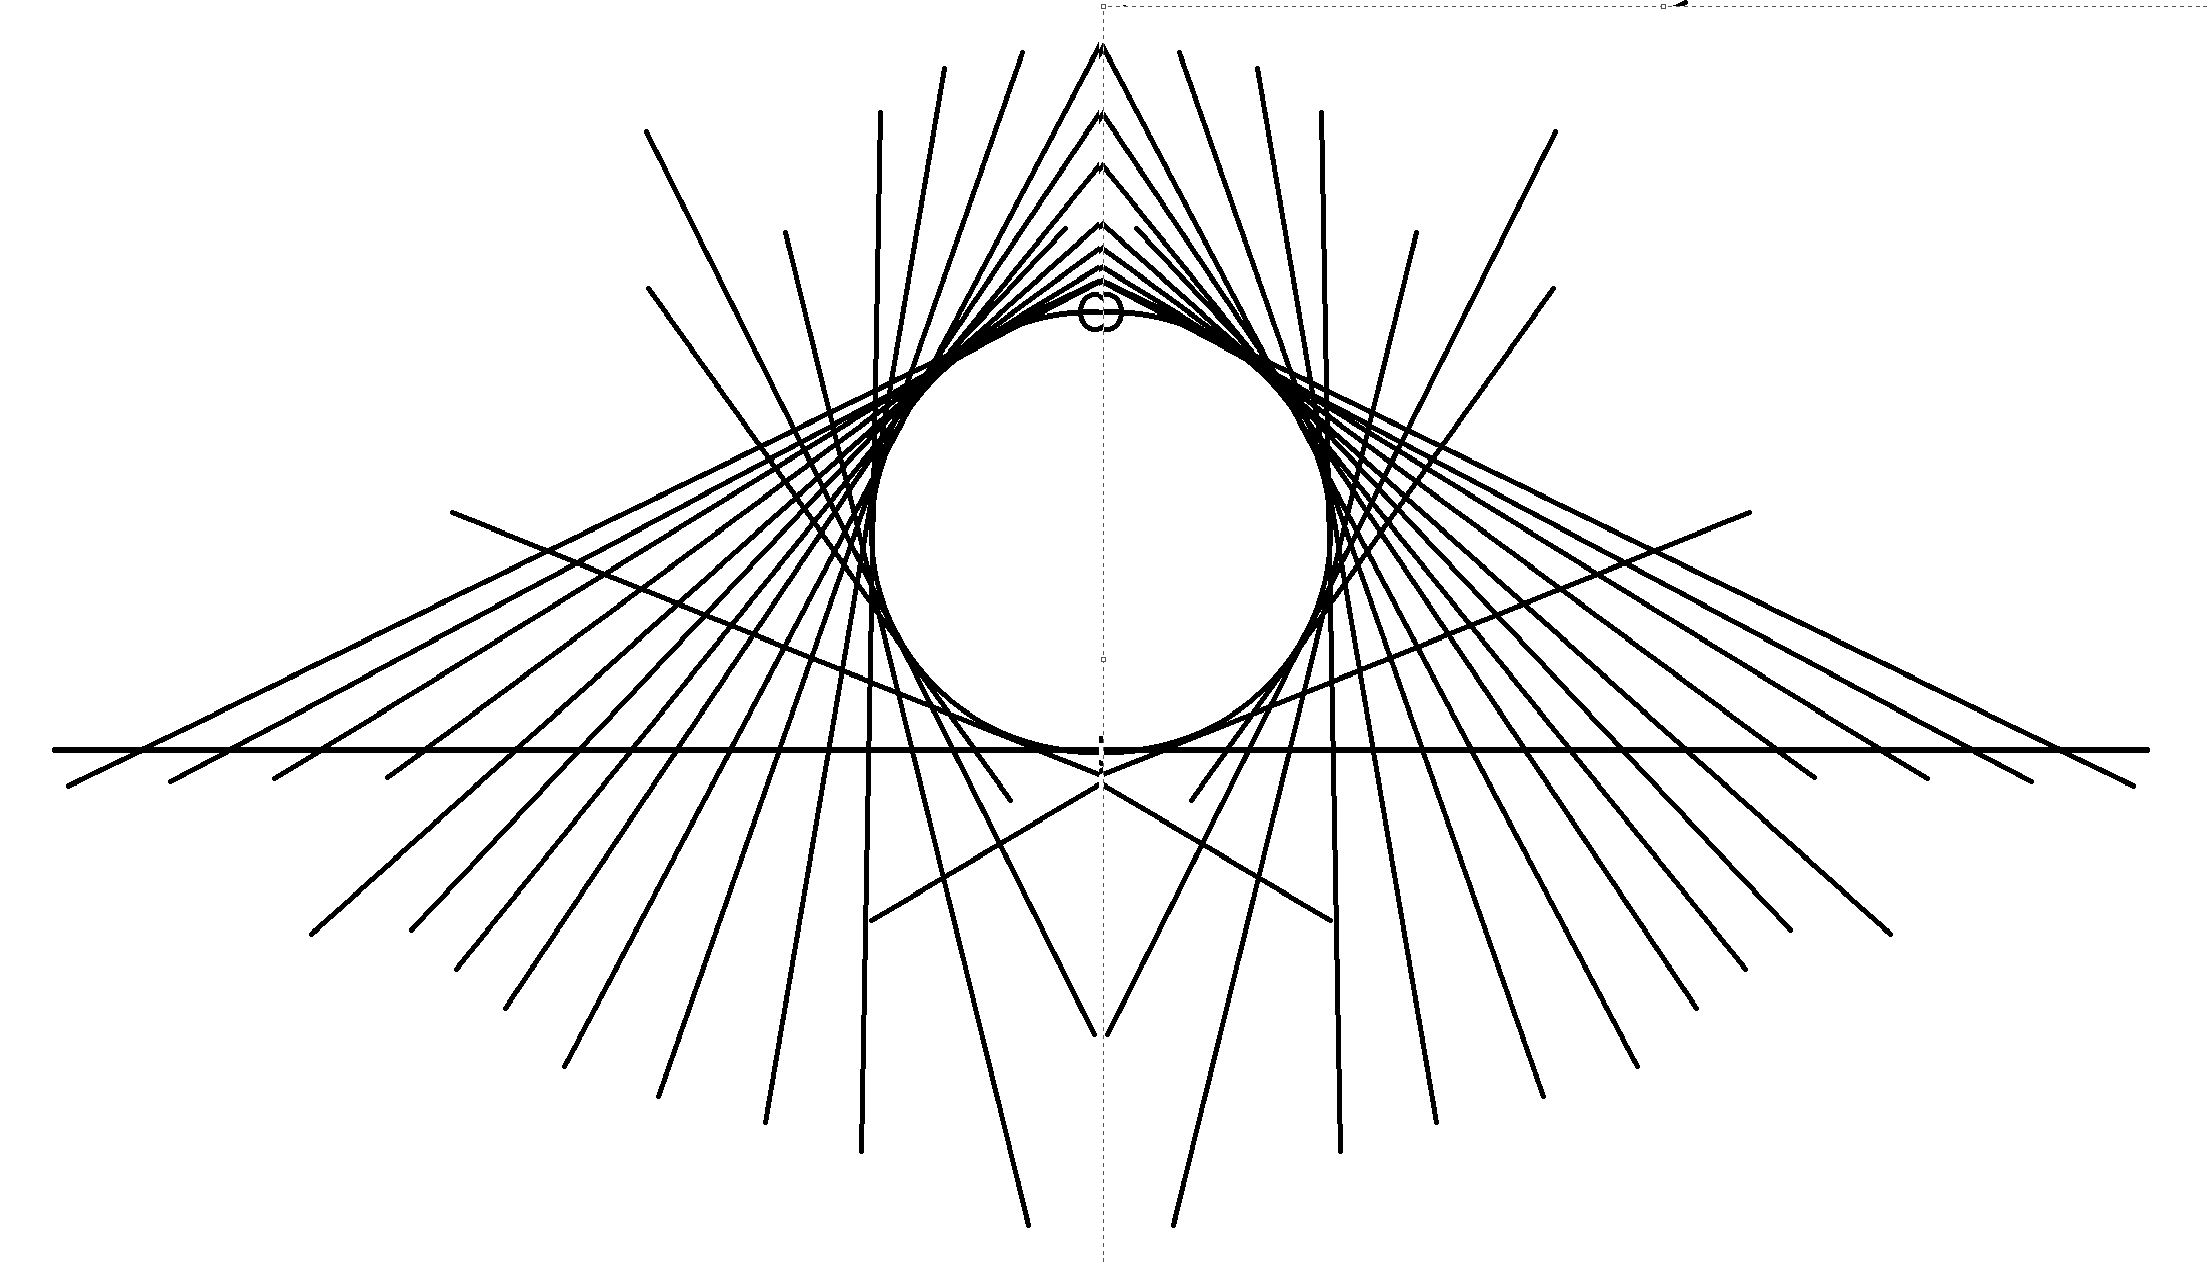
\includegraphics[scale=0.5]{notebook/topology_circle.png}}
\caption{a visual proof}
\label{fig}
\end{figure}


\fbox{Theorem 8.1} (1-3) The following are equivalent:
\begin{enumerate}
    \item $X$ is connected
    \item There is no continuous function $f:X\rightarrow \R_{std}$ such that $f(X) = \{0,1\}$.
    \item $X$ is not the union of two disjoint non-empty seperated sets.
\end{enumerate}
\fbox{proof}
We will first prove that 1 implies 2. Suppose that $X$ is connected. Suppose by way of contradiction that there is in fact a continuous function $f:X\rightarrow \R_{std}$ such that $\R$ is $f(X) = \{0,1\}$. Since $\{0\}$ is closed in the standard topology we know that $\R-\{0\}$ is open. Hence it's preimage must be open in $X$. Likewise, the preimage of $\R-\{1\}$ must be open in  $f$. Suppose by way of contradiction that $f^{-1}(\R-\{0\})$ and $f^{-1}(\R-\{1\})$ share some element $x$. Then $f(x) \in \R-\{0\}$ and $f(x)\in \R-\{1\}$. But since $f(X) = \{0,1\}$ and $x\in X$, $x$ must be $0$ or $1$, but it is neither because it's in $\R-\{0\}$ and $\R-\{1\}$. Hence $f^{-1}(\R-\{0\})$ and $f^{-1}(\R-\{1\})$ must be disjoint. But since they must also be open, and since they must make up all of $X$, it follows that $X$ is not connected, contradicting the assumption that it is. \\

Now we will prove that 2 implies 3. Suppose by way of the contrapositive that $X$ is the union of two disjoint non-empty seperated sets. Call these sets $A$ and $B$. Consider the function $f:X\rightarrow \R$ which maps elements of $A$ to $1$ and elements of $B$ to $0$. Since $A$ and $B$ are seperated, $A$ cannot contain any of the limit points of $B$, and vice versa. Because they partition $X$, it follows that both $A$ and $B$ must be closed. Furthermore, $X-A= B$, hence $B$ is open, and likewise for $A$. Consider an arbitrary open set $U$ in $\R_{std}$. Then there are two cases: (1) $U$ contains both 1 and 0, (2) $U$ contains one but not the other, and (3), $U$ contains neither 1 nor 0. In the first case the preimage is $X$, which is open. In the second case, the preimage is either $A$ or $B$, both open. In the third case the preimage is $\emptyset$, which is open. So open sets in $\R_{std}$ are mapped to by open sets in $X$, and $f$ is continuous.\\

Now we will prove that 3 implies 1. Suppose that $X$ is not the union of two disjoint non-empty sets. Then $X$ is not the union of two disjoint non-empty open sets, because disjoint non-empty open sets are disjoint non-empty sets. So $X$ is connected.\\

Having proven that $1\rightarrow 2\rightarrow 3\rightarrow 1$, the whole thing collapses logically into equivalence.
Q.E.D.
\end{document}
